% Chapter 1

\chapter{Evaluation and Comparison} % Main chapter title

\label{Chapter4} % For referencing the chapter elsewhere, use \ref{Chapter1} 

%----------------------------------------------------------------------------------------

% % Define some commands to keep the formatting separated from the content 
% \newcommand{\keyword}[1]{\textbf{#1}}
% \newcommand{\tabhead}[1]{\textbf{#1}}
% \newcommand{\code}[1]{\texttt{#1}}
% \newcommand{\file}[1]{\texttt{\bfseries#1}}
% \newcommand{\option}[1]{\texttt{\itshape#1}}

%----------------------------------------------------------------------------------------

With reference to the three research questions posed in chapter \ref{Chapter1}, this project aims to provide researchers with a simple to use, non-technical platform with which to move workflows and research environments to where the data they intend to process is located, through the use of cloud and container technology. Nikeza aims to act as a middleman to facilitate the specification of research environments for a workflow and allow the cloud environment to execute the researchers' pipeline without manual intervention. 

Nikeza needs to be compared to an alternative that is currently being used to process remote data. As mentioned in the Local Approaches subsection of the Related Work chapter, SANBI utilises remote processing locations to do some analyses already. One of the popular choices is using a cloud environment, Amazon Elastic Compute Cloud (EC\textsuperscript{2}) to be specific. The following section will detail the comparison of executing an identical workflow remotely on Amazon EC\textsuperscript{2}, which is through use of the US-east-2 (Ohio) data center and OpenStack, which is running in a lab environment set up by the University of the Western Cape Internet Communication Services department, with Nikeza running on top of it.

The evaluation here forth will assume that the Nikeza system is already installed and made available to the user, as the installation and maintenance of the actual software system is not part of the point that this thesis paper sets out to demonstrate, but rather the use of said system.

\section{Outline}

\subsection{Task}

The task for each system is to execute a Fastqc\footnote{Fastqc is a tool which provides simple quality control checking for raw sequence data.} workflow written in the Common Workflow Language, which takes advantages of tools packages into Docker containers. The full execution command is shown in Listing \ref{lst:cwl-Fastqc}.

\begin{lstlisting}[language=bash,caption={The command specified to execute the Fastqc workflow.}\label{lst:cwl-Fastqc}]
cwl-runner fastqc.cwl --INPUT SRR5439551.fastq --nofilter --nogroup --quiet
\end{lstlisting}

The CWL workflow simply specifies that the Fastqc tool, packaged in the \url{quay.io/ncigdc} Docker image, should be run with the following arguments:

\begin{itemize}
    \item \texttt{-{}-}INPUT SRR5439551.fastq
    \begin{itemize}
        \item The input data to use, SRR5439551.fastq in this case.
    \end{itemize}
    \item \texttt{-{}-}nofilter
    \begin{itemize}
        \item Retains all reads in the output report.
    \end{itemize}
    \item \texttt{-{}-}nogroup 
    \begin{itemize}
        \item Disable grouping of bases for reads >50bp in order to show data for every base in the read.
    \end{itemize}
    \item \texttt{-{}-}quiet 
    \begin{itemize}
        \item Reduce output from the Fastqc program during execution.
    \end{itemize}
\end{itemize}

The actual workflow being used in this test is not of any real importance. The goal was to generate a result (the output data of a workflow) from an arbitrary workflow in order to prove whether Nikeza would work or not. The aforementioned workflow provided this result, by generating a small report of the data set. The task is not to determine whether workflow languages output reproducible results.

There were a number of assumptions made about the testing environments before the tests are performed. This is detailed in table \ref{tab:assumptions}.

\begin{table}[ht!]
\centering
\caption[Cloud Environment Assumptions]{Assumptions of the testing environments for OpenStack with Nikeza and AWS platforms.}
\label{tab:assumptions}
\resizebox{\textwidth}{!}{%
\begin{tabular}{p{0.5\linewidth}p{0.5\linewidth}}
\toprule
OpenStack                                                                                         & Amazon AWS                                                                                            \\ \midrule
A user account with limited standard privileges is created for the test.                          & A user account with standard privileges is created for the test.                               \\ \midrule
A Swift container is created for the test data-set to be stored on.                               & A Simple Storage Service (S3) "bucket" is created for the test data-set to be stored on.       \\\midrule
A Swift container is created for the result data to be stored on after the analysis is completed. & An S3 "bucket" is created for the result data to be stored on after the analysis is completed. \\\midrule
Both containers are made available to the test user.                                              & Both S3 "buckets" are made available to the test user.                                         \\\midrule
Test user virtual machines are allowed to access the internet.                                    & Test user virtual machines are allowed to access the internet.    
\\ \bottomrule
\end{tabular}%
}
\end{table}

\subsection{Data set}

For the testing, the so-called "Genome In A Bottle" data set was used. This data set includes reads from NA12878 and is a very well-studied and classified \parencite{paajanen2017critical}. It was chosen due to it being a manageable and relatively small set of data in order for testing and iteration on the project. 

As mentioned with the previous section, the goal is only to perform some arbitrary task and to then compare the work required to set up the analysis environment manually against the work required to use the proposed solution. As such, only the above data set was chosen to test the methodology for this project. The result of the processing on this data set will be different for different workflows, but each workflow should output reproducible results given the nature of workflow languages.

\subsection{Metrics}

\subsubsection{Number of actions for the user to perform in order to set up the workflow environment.}
The working environment for the workflow includes preparing the computer system that will be running the analysis. The operating system needs to be installed, software dependencies need to be installed on top of that operating system and data needs to be made available from the data storage of the remote environment into the working environment.

\subsubsection{Number of actions for the user to perform in order to retrieve the data from the remote environment into the workflow environment.}
Data movement still occurs in some capacity. While the data is present at the remote site, it is stored in an object store. The data needs to be copied from the object store into the computing system that is to be used for the analysis.

\subsubsection{Number of actions for the user to perform in order to execute the workflow.}
The amount of actions that need to be performed in order to start and complete the analysis on the selected data.

\subsubsection{Number of actions for the user to perform in order to retrieve the processed data.}
Once the analysis is complete the data needs to be made available to be retrieved by the person who intends to use it.

\section{Results}
This section will detail the process of testing and the results of these tests. It showcases the technical steps involved in both systems, Amazon AWS and OpenStack with Nikeza, to provide perspective on how complex and time consuming using cloud environments directly can be. This is especially important in cases where researchers are not technically proficient or in an environment where the technical expertise are available.

The "Genome in a Bottle" data set was processed with a simple Fastqc workflow using both the OpenStack with Nikeza system as well as the Amazon AWS platform. 

\subsection{Amazon AWS}

\subsubsection{Pre-work}

Two S3 buckets were created on the SANBI Amazon AWS account:

\begin{itemize}
    \item eugene.masters.data; the container that would host the data set as if it were already present on the remote system. This bucket was created on the U.S. East (Ohio) data center (Figure \ref{fig:s3_buckets}).
    \item eugene.masters.result; the container that would host the results of the researcher workflow on the remote system. This bucket was created on the U.S. East (Ohio) data center (Figure \ref{fig:s3_buckets}).
\end{itemize}

\begin{figure}[h!]
\centering
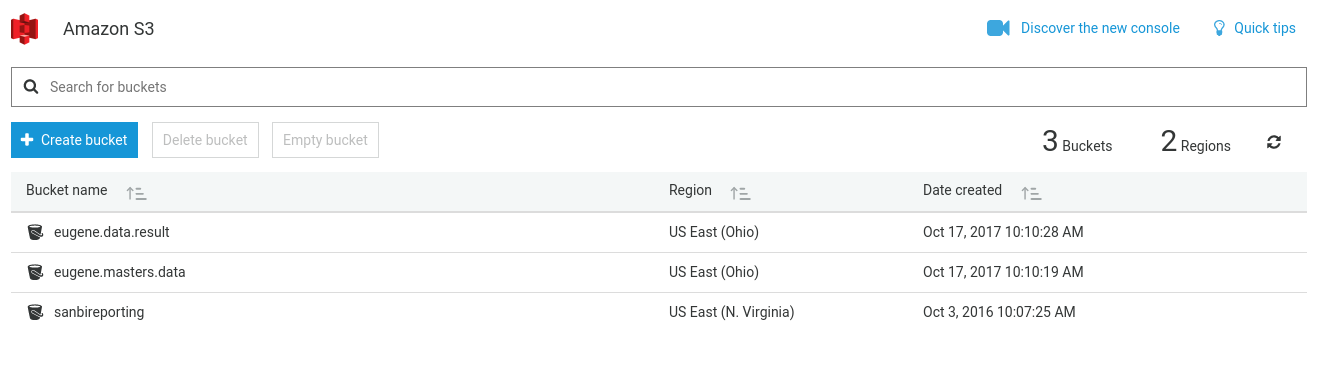
\includegraphics[width=\textwidth]{Figures/4_s3_buckets.png}
\decoRule
\caption[AWS S3 Buckets for Testing]{This figure shows the S3 buckets created for the SANBI workspace on Amazon AWS.}
\label{fig:s3_buckets}
\end{figure}

The data set (SRR5439551.fastq) was first uploaded to the eugene.masters.data bucket. This allowed it to be accessible to virtual machines that intend to use the data.

\subsubsection{Process}

The user logged into the AWS dashboard. From here, they navigate to the EC2 (Elastic Compute Cloud) dashboard. The user selected the Instances tab, followed by the "Launch Instance" button. Here, the user was presented with a list of virtual machine images to select, shown in Figure \ref{fig:aws_ami}.

\begin{figure}[h!]
\centering
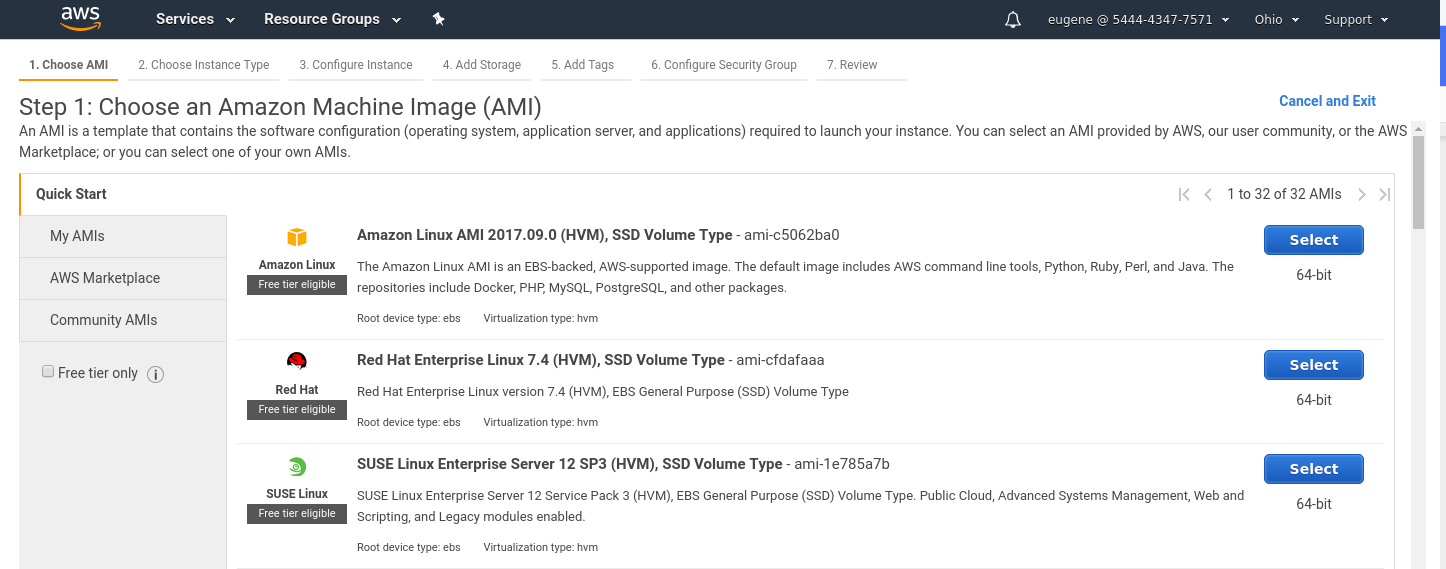
\includegraphics[width=\textwidth]{Figures/4_aws_select_instance.png}
\decoRule
\caption[List of Amazon Machine Images Available on AWS]{This figure shows the list of AMI (Amazon Machine Image) the user can choose from on the Amazon AWS web interface.}
\label{fig:aws_ami}
\end{figure}

In this case, the user would normally select whichever operating system is dictated to them or recommended by their institution. For the proof-of-concept, the Red Hat Enterprise Linux 7.4 (HVM), SSD Volume Type AMI was selected.

The next step involved selecting the instance type, which determines the hardware resource availability that is granted to the virtual instance. This is also generally dictated to the user by their institution. For proof-of-concept purposes, the General Purpose t2.micro instance was chosen. This instance type has 1 virtual CPU core and 1GB of memory available to it. The user selected the "Review and Launch" button. From the review screen, the "Launch" button was pressed and the user was presented with a screen that asked which key-pair to use for secure remote access to the virtual machine operating system environment via SSH. A new key-pair was generated in this case called eugene.masters and it was downloaded onto the computer the test was done from, shown in Figure \ref{fig:aws_keypair}.

\begin{figure}[h!]
\centering
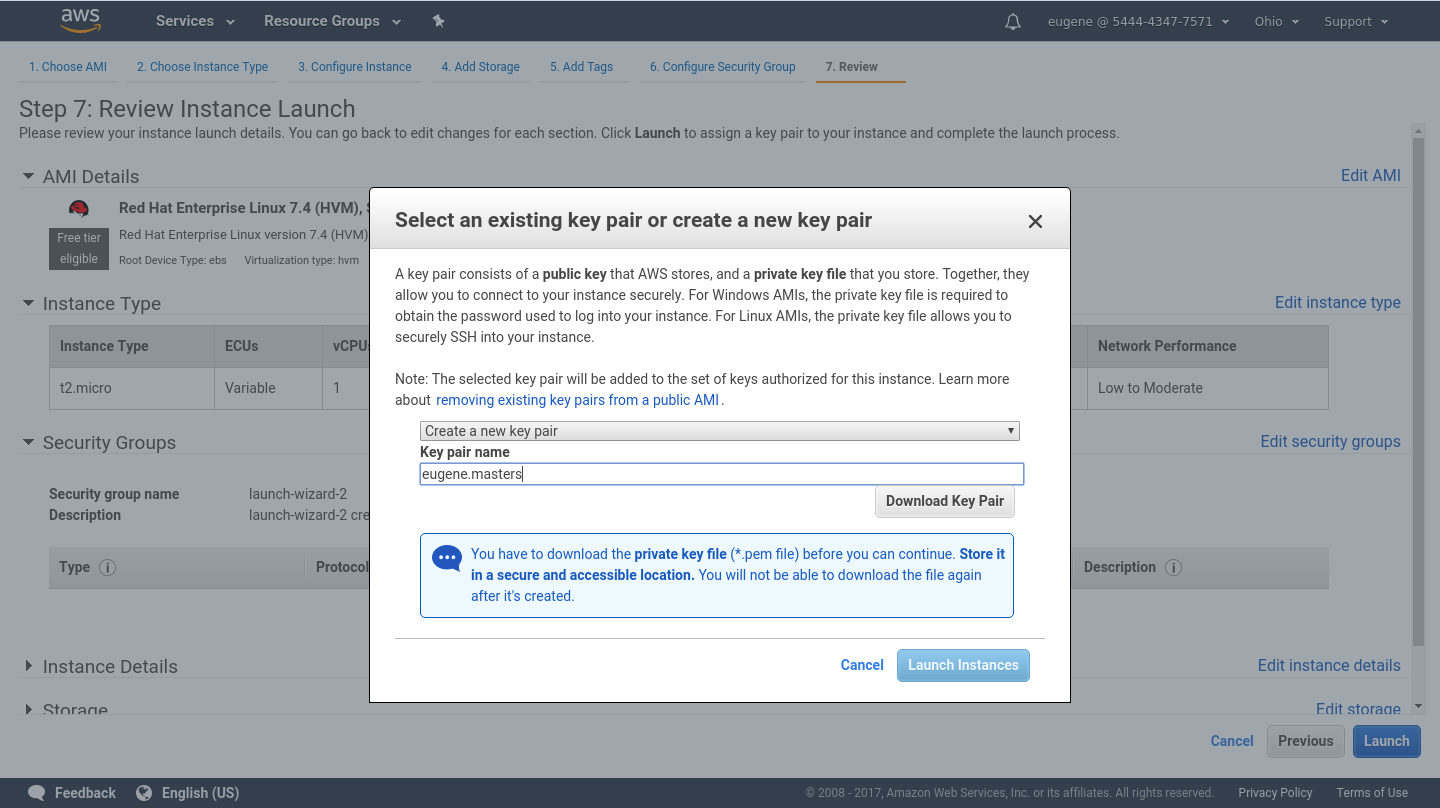
\includegraphics[width=\textwidth]{Figures/4_aws_keypair.png}
\decoRule
\caption[AWS Keypair Creation]{Demonstration of creating a key-pair to use for securely accessing the virtual instance.}
\label{fig:aws_keypair}
\end{figure}

Once the launch button was pressed by the user, they navigated back to the Instances tab in order to retrieve their IP address for accessing the virtual machine. The IP address is available from the dashboard as illustrated on the right of Figure \ref{fig:aws_instancelist}. 

\begin{figure}[h!]
\centering
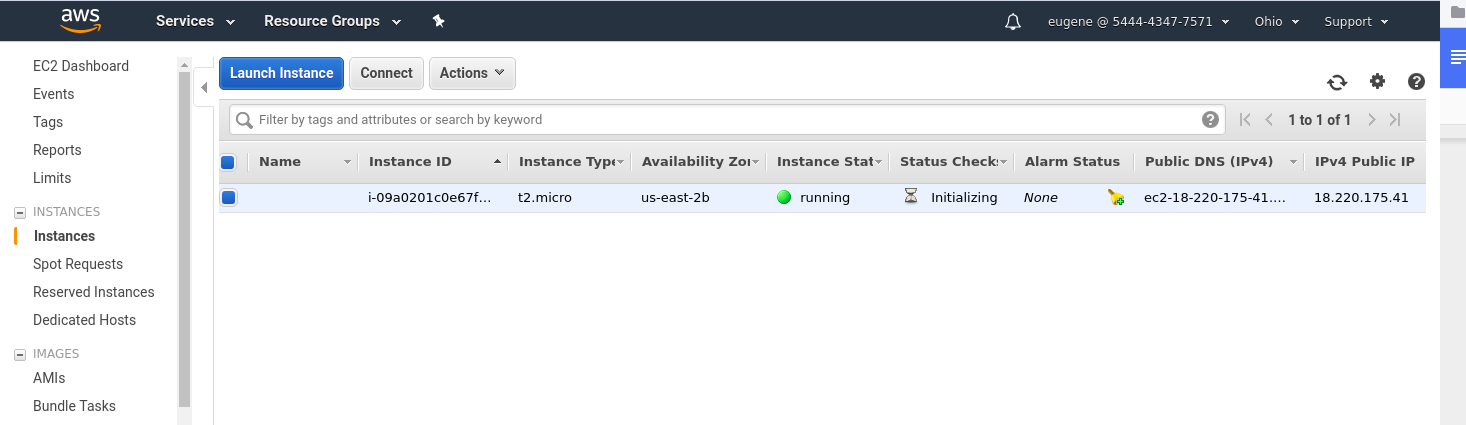
\includegraphics[width=\textwidth]{Figures/4_aws_instancelist.png}
\decoRule
\caption[AWS Instances View]{This is the Instances tab on the Amazon AWS web interface for the user, where the public IP address is retrieved.}
\label{fig:aws_instancelist}
\end{figure}

The user was required to change the permission of the keyfile that was downloaded from AWS when creating the instance to Unix permission set 400 if on Linux, or use an SSH client such as PuTTY on Windows. The user then created an SSH session into the virtual environment via the command shown in Listing \ref{lst:ssh}.

\begin{lstlisting}[language=bash,caption={Utilising the key in order to access a remote terminal session in the new virtual instance.}\label{lst:ssh}]
ssh -i eugenemaster.pem ec2-user@18.220.175.41
\end{lstlisting}

Running this command provided the user with a bash terminal inside of the virtual machine hosted by Amazon.

For the user to be able to retrieve data from an S3 bucket, they needed to ensure that the tool being used to do so could authenticate the user. The user retrieved the Access Key ID associated with their account under the Users dashboard in the AWS console by selecting "Create Access Key" after which they took note of the ID and the secret key.

In order for the user to retrieve the data from the AWS S3 bucket, they were required to download it into the running instance. This was done through Amazon supplied CLI tools that were installed to the container. This step could have also been accomplished using standard Linux tools, but introduce additional complexity. First, the user navigated to the S3 dashboard in order to retrieve the endpoint and location of the data on the S3 bucket. The AWS CLI tool was installed onto the virtual instance. In order to do this, the user executed the command shown in Listing \ref{lst:aws_cli_install}.

\begin{lstlisting}[language=bash,caption={Utilising the key in order to access a remote terminal session in the new virtual instance.}\label{lst:aws_cli_install}]
sudo easy_install awscli
\end{lstlisting}

This installed the AWS CLI tool onto the virtual instance using the Python package manager. The Python installation method is the simplest and quickest way to get this tool running in this case. Once complete, the user configured their credentials by executing the command shown in Listing \ref{lst:aws_conf}.

\begin{lstlisting}[language=bash,caption={Setting up the initial AWS tool configuration.}\label{lst:aws_conf}]
aws configure
\end{lstlisting}

Here the user entered the Access Key ID, Secret Access Key, region that the data exists on (us-east-2 in this case) and output format, after which they executed the command in Listing \ref{lst:aws_s3_cpy}.

\begin{lstlisting}[language=bash,caption={Using the AWS tool to copy the data from the S3 bucket to the virtual instance.}\label{lst:aws_s3_cpy}]
aws s3 cp s3://<bucket name>/<file name> .
\end{lstlisting}

In this case the bucket name was eugene.masters.data and the file name SRR5439551.fastq, which is the data that was to be processed. This command will copy the data from the cloud provider's storage to the storage that the virtual instance has access to.

Once the data was on the virtual instance, the user installed the tools necessary for executing the workflow. For the Fastqc workflow sample, this was Docker and cwl-runner. With Red Hat Enterprise Linux (RHEL), Python version 2 is shipped by default. cwl-runner requires Python version 3, however this does not exist in the default RHEL repositories. A custom repository needed to be added in order to install cwl-runner, shown in Listing \ref{lst:aws_setup_os}.

Once completed, the other dependency for the workflow needed to be installed. Docker is also not contained in the repositories for RHEL and as a result the steps on the Docker website were followed in order to install it: \url{https://docs.docker.com/engine/installation/linux/docker-ee/rhel/}. Once Docker was installed, the daemon process was enabled and started as shown in Listing \ref{lst:aws_docker}.

\begin{minipage}{\linewidth}
\begin{lstlisting}[language=bash,caption={The steps for adding the repository to RHEL for retrieving Python 3 and cwl-runner.}\label{lst:aws_setup_os}]
sudo rpm -ivh \ https://dl.fedoraproject.org/pub/epel/epel-release-latest-7.noarch.rpm
sudo yum -y install https://centos7.iuscommunity.org/ius-release.rpm
sudo yum -y update
sudo yum -y install python36u python36u-setuptools
sudo easy_install-3.6 cwl-runner
\end{lstlisting}
\end{minipage}

\begin{lstlisting}[language=bash,caption={Enabling and starting the docker service.}\label{lst:aws_docker}]
sudo systemctl enable docker && sudo systemctl start docker
\end{lstlisting}

Now the cwl workflow was uploaded to the instance using scp. Any other tool which allows the workflow to be moved could also have been used. 

For RHEL specifically, in order to execute the workflow the user needed to disable SELINUX on the operating system. This was done through changing the "enforcing" line to "disabled" in the file /etc/selinux/config. If this is not done, cwl-runner would not have been able to write output to the file system of the operating system and would have failed as a result. The virtual instance was rebooted for changes to take effect. Once rebooted, the user executed the workflow as shown in Listing \ref{lst:aws_cwl_exec}.

\begin{lstlisting}[language=bash,caption={Executing the workflow on RHEL with cwl-runner installed and data copied.}\label{lst:aws_cwl_exec}]
sudo cwl-runner fastqc.cwl --INPUT SRR5439551.fastq --nofilter --nogroup --quiet
\end{lstlisting}

Once the process was complete, the user received a message "Final process status is success" from the tool, after which the user was then able to retrieve the output file from the virtual machine whichever way they wish, for example downloading it through scp directly from the virtual machine or uploading it to an s3 bucket as in this case. The data was uploaded to the eugene.masters.result bucket. Once the upload succeeded, the user could navigate to the S3 dashboard, select the bucket and download the data from there as shown in Figure 6.5.

\begin{figure}[h!]
\centering
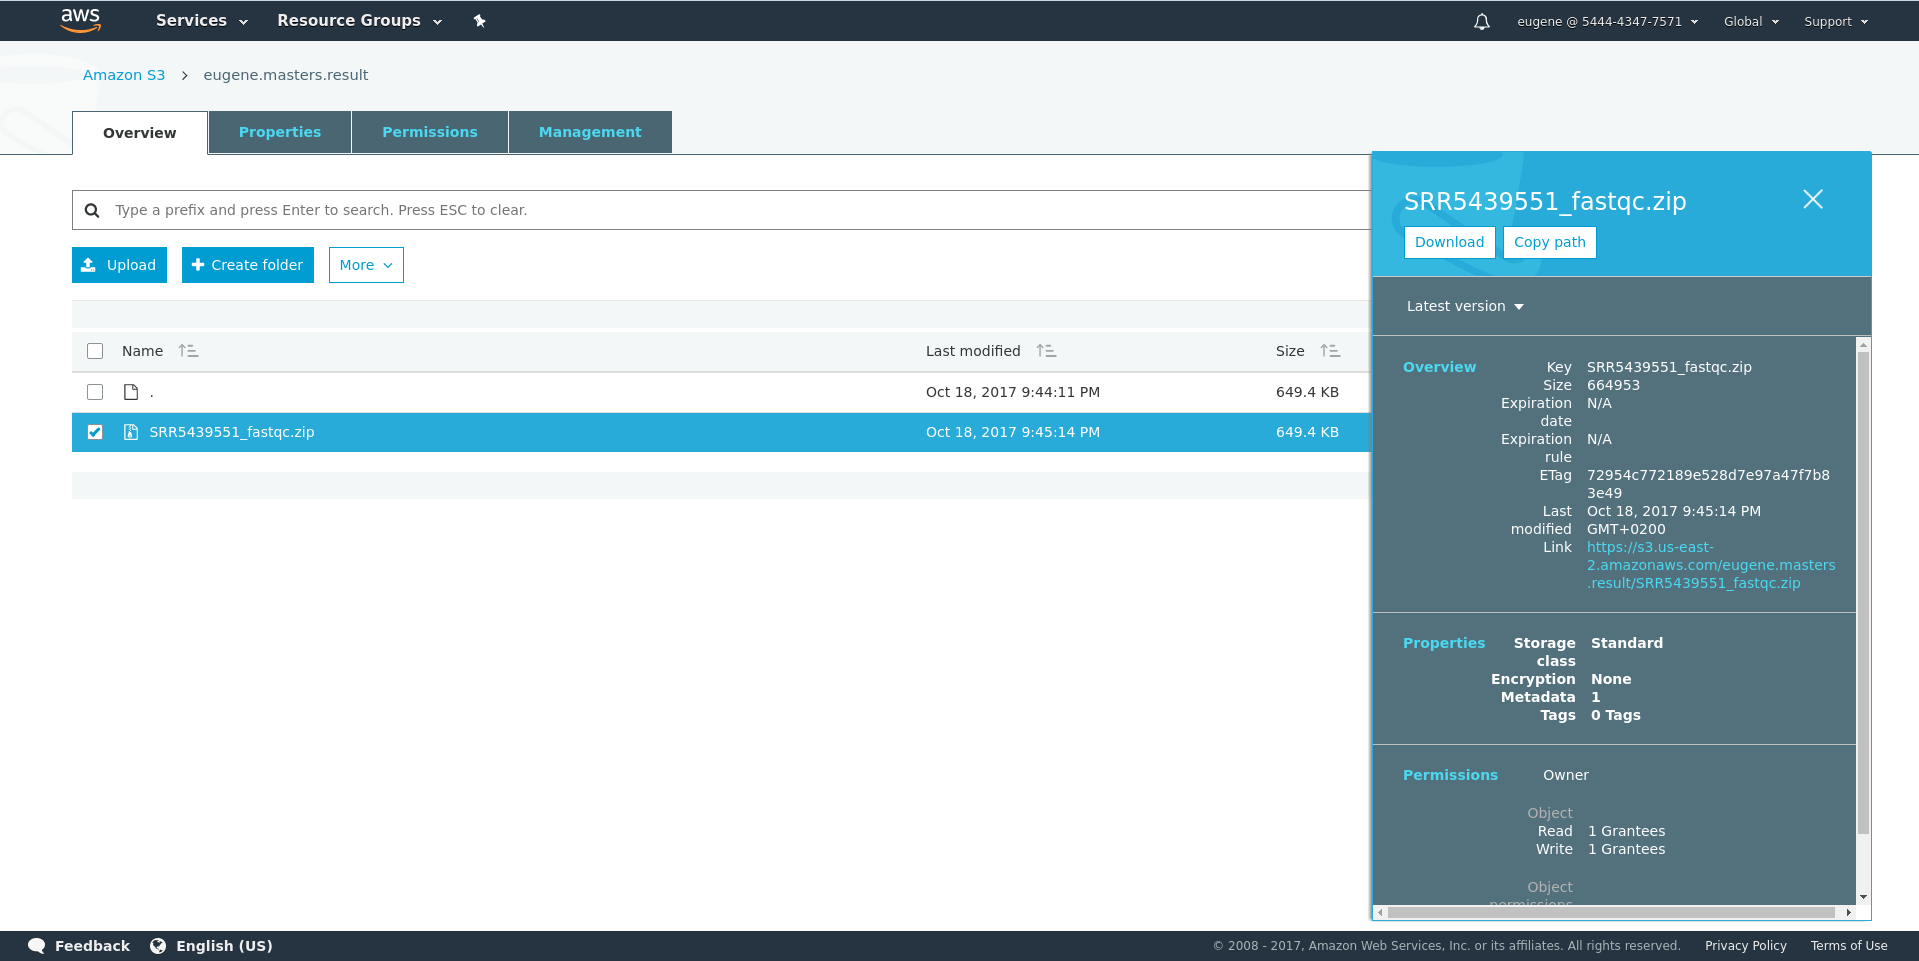
\includegraphics[width=\textwidth]{Figures/4_s3_bucket_result.png}
\decoRule
\caption[AWS S3 Bucket with Result Data]{This shows the data generated from the workflow stored in the eugene.masters.result S3 bucket.}
\label{fig:aws_s3_result}
\end{figure}

\subsection{OpenStack with Nikeza}

\subsubsection{Pre-work}

Two Swift containers were created on the OpenStack backend for the test user.

\begin{itemize}
    \item seqdata; the container that would host the data set as if it were already present on the remote system (Figure \ref{fig:swift_prep}).
    \item resultant; the container that would host the results of the researcher workflow on the remote system (Figure \ref{fig:swift_prep}).
\end{itemize}

\begin{figure}[h!]
\centering
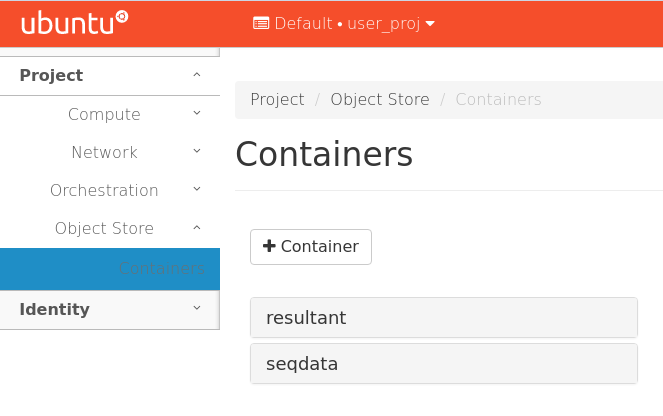
\includegraphics[width=\textwidth]{Figures/4_os_swift_prep.png}
\decoRule
\caption[OpenStack Swift Containers for Testing]{This shows the data containers created in Swift in the OpenStack system for the user.}
\label{fig:swift_prep}
\end{figure}

\subsubsection{Process}

The data set (SRR5439551.fastq) was first uploaded to the eugene.masters.data bucket. This allowed it to be accessible to virtual machines that indent to use the data.

With the Nikeza system in place, a user needs to navigate to the website that provides the Nikeza interface. Here the user was presented with a login screen on which they must enter their credentials for the cloud environment of that institution (provided to them through that institution or based on federated authentication). This screen is shown in Figure \ref{fig:os_login}.

\begin{figure}[h!]
\centering
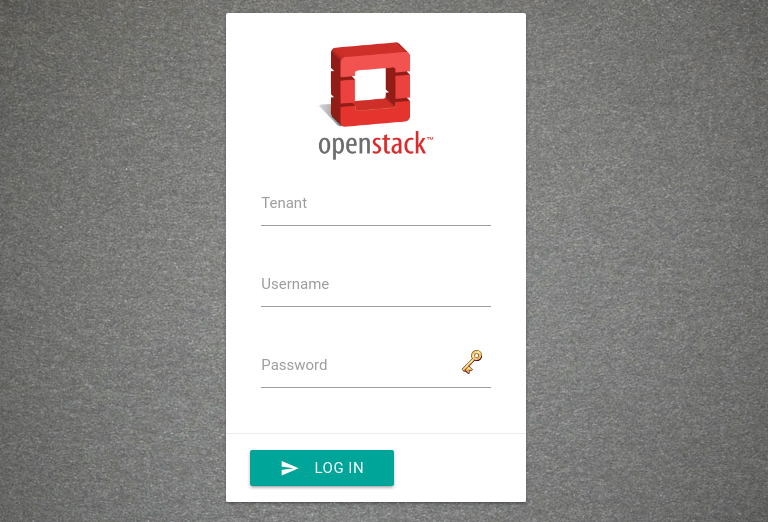
\includegraphics[width=\textwidth]{Figures/4_os_login.png}
\decoRule
\caption[Nikeza Login Screen]{This image shows the Nikeza login screen configured with OpenStack backend.}
\label{fig:os_login}
\end{figure}

Once the user was logged in, they were provided a dashboard which showed their queued and running jobs shown in Figure \ref{fig:os_queue}. There were no active jobs for the user. Two buttons below the queue are shown, one to create a new job and one to stop any selected jobs.

\begin{figure}[h!]
\centering

\includegraphics[width=\textwidth]{Figures/4_os_queue.png}
\decoRule
\caption[Nikeza Job Queue Page]{The Nikeza queue page with no active jobs.}
\label{fig:os_queue}
\end{figure}

The user clicked the button to create a new job. As shown in Figure 6.9, the page that they were provided with asked the user to upload the workflow file that they would have written or retrieved from another source, fastqc.cwl in this case, followed by the arguments for the workflow shown in Listing \ref{lst:os_cwl_comm}.

\begin{lstlisting}[language=bash,caption={The arguments for the workflow in question.}\label{lst:os_cwl_comm}]
--INPUT SRR5439551.fastq --nofilter --nogroup --quiet
\end{lstlisting}

The user then selected the data they wish to process from a list provided to them in the second step box, they selected the directory in the virtual machine that the data would be placed, or copied, in step 3 and where the resultant data would be created in the virtual machine in step 4 and finally which container the user wants the data to be uploaded to the cloud environments storage solution.

\begin{figure}[h!]
\centering
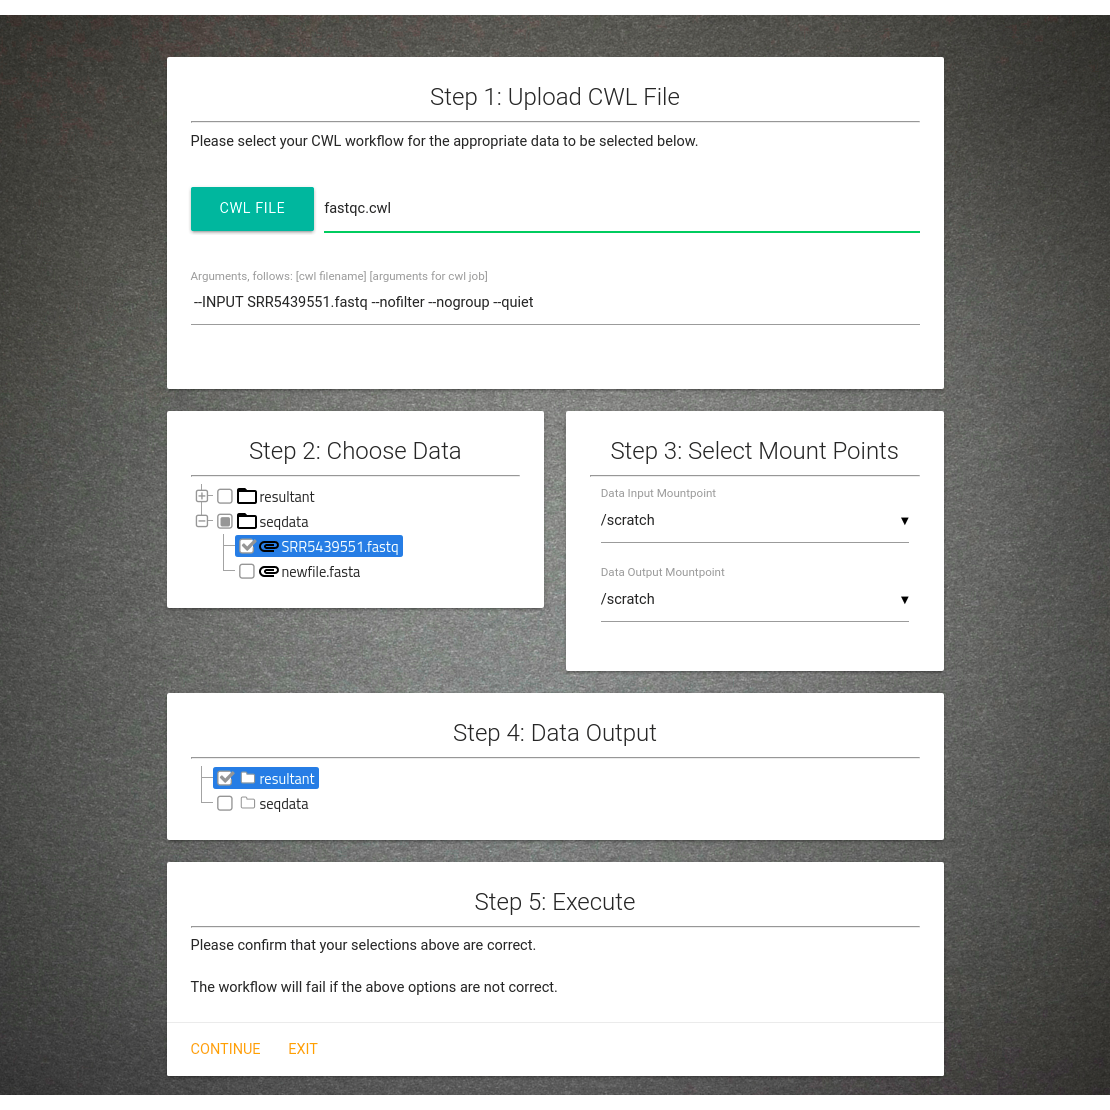
\includegraphics[width=\textwidth]{Figures/4_os_config.png}
\decoRule
\caption[Nikeza Workflow Configuration Screen]{The Nikeza workflow creation and configuration page, where the user will select the CWL file they wish to execute and the details around the workflow.}
\label{fig:os_conf}
\end{figure}

The user clicked the button to start the workflow (CONTINUE) and waited on the processing to finish. Once the workflow was completed the data was uploaded to the container specified by the user, the resultant container in this case, and the virtual machine was destroyed. The user could now fetch the data from the resultant container, shown below in Figure \ref{fig:os_result}.

\begin{figure}[h!]
\centering
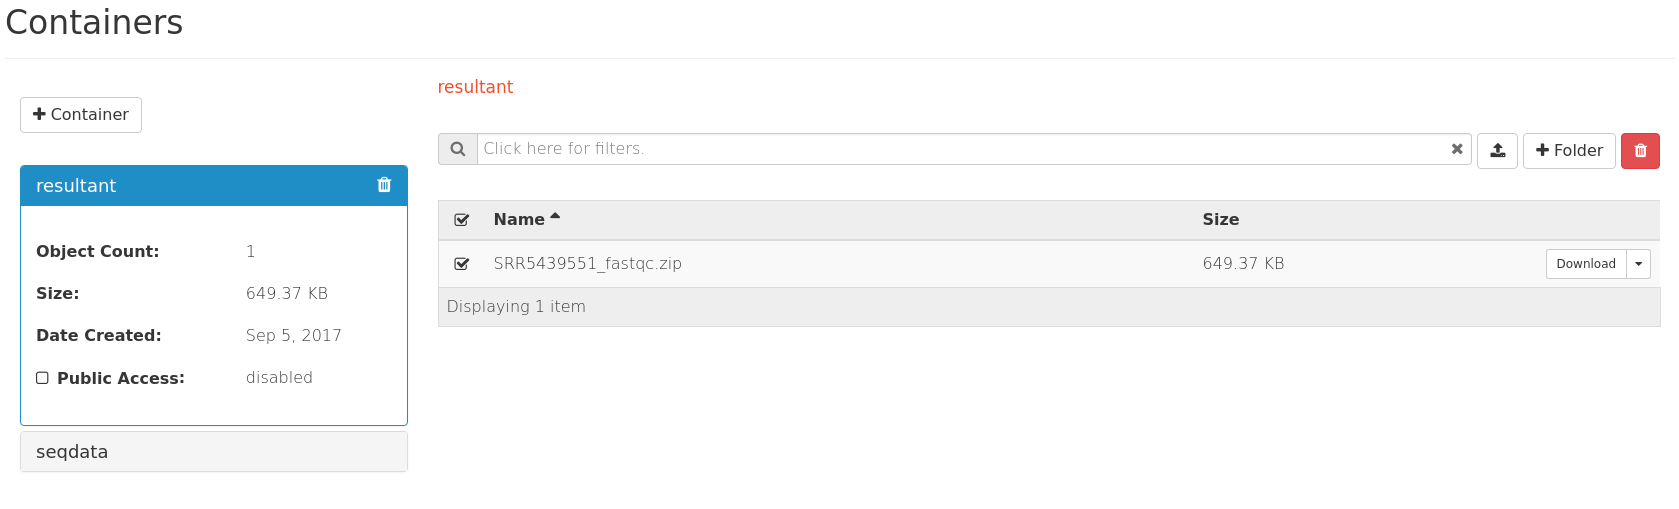
\includegraphics[width=\textwidth]{Figures/4_os_swift_result.png}
\decoRule
\caption[OpenStack Swift Container with Result Data]{This shows the data generated from the workflow stored in the resultant OpenStack container.}
\label{fig:os_result}
\end{figure}

\subsection{Summary}

It should be clear that from a user perspective, using the cloud directly involves a substantial amount of additional work than using something such as the project demonstrated in this thesis. The below sections summarise the differences (also see Table \ref{tab:comparison_overview}).

\subsubsection{Amazon AWS}
The user must navigate to the website and log in with their credentials for the cloud provider. They must then navigate to the correct tab where they can create instances (virtual machines) to run their work. Once there, they can create a virtual machine by selecting the image type that hey want followed by the instance type. If the user has already created a key pair then they may select to use that or to create a new key pair, otherwise they will be prompted to create a key pair for the instance. Assuming no key pair was created prior to the creation of the virtual machine instance, the user must then download the newly created key pair and set the correct permission on the file. They can now log into the instance via an IP address shown to them in the instance menu on the cloud dashboard. Once inside, they can install the cloud provider tools to access the data storage, configure the tools with their account details and download the data onto the running instance. Before running the workflow, they must ensure that Docker is installed and activated and that a CWL executor is installed onto the instance. They can then safely start the workflow.

When the workflow completes, the user must upload the data from the instance to the cloud storage of the provider using the same method of retrieving the raw data. Once complete they will be able to retrieve the results from the storage page on the cloud provider dashboard.

The last step for the user is to shut off the running virtual instance.

\subsubsection{Nikeza}
The user must navigate to the Nikeza dashboard and log in with their provided cloud credentials. Once logged in, they can click the "Add" button on the page they are presented with. The next page presents then with a form where they can select the workflow file from their local computer, specify the arguments for the workflow and select the data they want to process. After completing the form, the user clicks the "CONTINUE" button. The workflow environment is now being prepared and the workload is being executed in the background automatically.

When the workflow completes, the user will be able to retrieve the results from the storage page on the dashboard of the cloud provider being used behind Nikeza. The virtual machine instance is shut down for the user.

\subsubsection{Overview}


% Please add the following required packages to your document preamble:
% \usepackage{booktabs}
\begin{table}[ht!]
\caption[Step Differences between Nikeza and Amazon AWS]{The differences between steps needed to complete the work task using OpenStack with Nikeza and Amazon AWS.}
\label{tab:comparison_overview}
\resizebox{\textwidth}{!}{%
\begin{tabular}{p{0.7\linewidth}p{0.15\linewidth}p{0.15\linewidth}}
\toprule
                                                                                                                                   & OpenStack with Nikeza & Amazon AWS \\ \midrule
Number of actions for the user to perform in order to set up the workflow environment.                                                           & 5                     & 15         \\ \midrule
Number of actions for the user to perform in order to retrieve the data from the remote environment into the workflow environment. & 0                     & 4          \\ \midrule
Number of actions for the user to perform in order to execute the workflow.                                                        & 1                     & 8          \\ \midrule
Number of actions for the user to perform in order to retrieve the processed data.                                                 & 3                     & 3          \\ \midrule
TOTALS                                                                                                                             & 9                     & 30         \\ \bottomrule
\end{tabular}
}
\end{table}

\section{Discussion}
For both of the aforementioned processes, the data that was generated was identical. The difference is in the ease and speed of actually executing the workflow that the researcher desires to do on the data set. While it is true that in both cases the data does not need to be moved from the cloud environments to the researcher first in order to do the work on it, assuming that the data was uploaded before hand, it is clear that one of the solutions is significantly more time consuming and technically involved. 

The Amazon AWS, or direct cloud, approach requires a greater deal of not only technical knowledge (depending on the virtual environment that the researcher is using), but also takes significantly longer to get into a state where the researcher is able to process their workflow. This can be mitigated by the cloud environment providing pre-built virtual images that contain the tools that a researcher would need, but this is not common and is also not manageable given all the novel requirements that various researchers have for their workflows.

The Nikeza system greatly simplifies the creation and dependency management of the virtual environment for the researcher. By providing the researcher with an intuitive and simple to follow interface for uploading their workflow and selecting their data set, the researcher is able to more rapidly submit workflows to be processed. It also reduces the need for a researcher to be reliant on additional personnel such as a technical person in order to assist them with creating the environment in the first place.

OpenStack itself was not tested separately due to the fact that it is very similar to how the user would engage with AWS. OpenStack exposes a very cloud-computing like dashboard to the end user if using Horizon (the OpenStack Dashboard system) directly. Due to this, the test between directly using OpenStack and Amazon AWS would result in mostly the same steps to be taken with some minor differences in syntax.
